% old Introduction stuff..
With this work we are exploring the ways in which sound and notifications can be
combined through the use of different types of intelligent agents and sound
scapes to create interfaces with differing goals.  We will explore the benefits
of context aware interfaces and the impact vocalization has on multi-tasking
environments. Figure 3.1 presents common examples of intelligent agents that
exist within visual interfaces that follow a similar paradigm.

\begin{figure}[h]
  \centering
  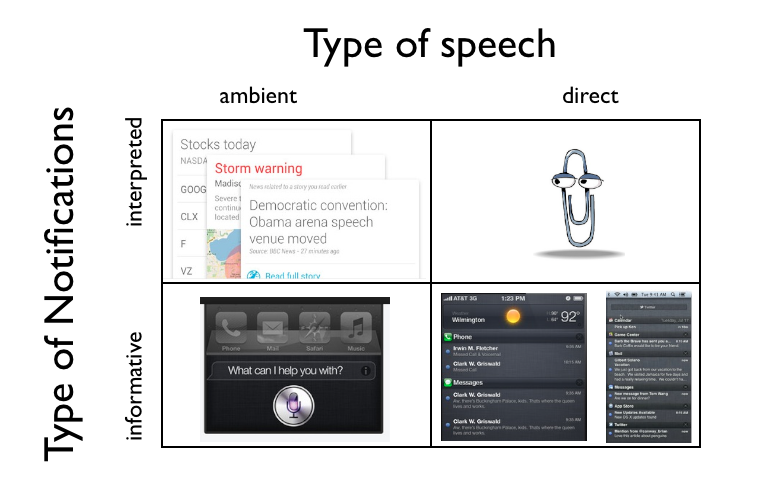
\includegraphics[width=1\textwidth]{images/chart.png}
  \caption{Visual examples of the types of interfaces we will explore in Auditory
  Interfaces}
\end{figure}

Formally, we are interested in four  aspects of these interfaces.

The most important question we pose looks at the ability of these interfaces to reduce
the users cognitive load. We describe auditory interfaces whose conceptual model
maps interface elements into a 3D audio space. The hypothises is that the extra dimension in the audio
can reduce the users cognitive load. As the four aformentioned interfaces use
binaural audio, we will explore thene features that allow audio and directionality
to reduce the cognitive load for the user. As these interfaces provide information to the user
in terms of spatial attenuation and audio feedback, we explore the added benefits
these new features can have on improving both the users comprehension of content
presented to them and their efficiency with interacting with the systems as they
provide users with cues to assist recall of information.

We then shift our focus to the role of audio in interface design.  Because of
sound's transient properties, its ability to portray or navigate through
interfaces elements changes.  More importantly, audible interfaces provide an
alternate mode of access to computers whenever a users’ visual focus is unavailable.
Visual focus can be unavailable for a number of reasons, such as when users are
driving, using hand-held devices while engaged in other physical activities that
command visual attention, or even as a result of physical disabilities~\cite{
michelis2008disappearing}. We are interested in understanding how a user's
interaction with sound can quantitatively be used to more efficiently accomplish
tasks in different scenarios.

Coupling sound with the intelligent agent drivers of the interface,  we raise
the question that asks to quantify the efficiency different types of intelligent
agent models have and how auditory interfaces can be used to complement the features
of these intelligent agents to encourage multi-tasking.

Finally, we will explore the decision making processes within each scope of
intelligent agent and audio scheme. With each type of stimuli or notification,
there is a stochastic decision that must be made regarding both the best manner
and the proper time to alert the user. In his work, Eric Horvitz quantified risks
and benefits of using different notification paradigms to express this
information. We explore how these trade offs present themselves in the auditory domain.




%%-----------------------------------------------------------------------------%
\section{                 Assistive Audio Interfaces                           }
% 2) audio used to assist user's comprehension      ~\cite{jeon2012listen2droom}

Work by researchers at Georgia Tech demonstrated the use of a single, radial axis
in an audio interface to present information to blind individuals. They presented
multiple user studies and work of assisting blind users navigate new or unfamiliar
rooms.  With smart phones and computer vision techniques the researchers in
Bruce Walker's Sonification lab created an application helping blind users understand
the orientation and placement of objects in new environments. Of note are the
current practices that blind users employ to navigate these settings. The focus group
Jeon et al. interviewed demonstrated that blind users employ
various strategies to place objects in a room such as one subjects summarization
that by "listening to the room, we can detect where running refrigerators,
computers, or other machinery exists" ~\cite{jeon2012listen2droom}. The second
most common response was that layout is also often inferred by touch, or assisted
navigation either with the use of inanimate objects (such as walking canes)
or sighted volunteers.

The smart phone application presented in this work allows visually handicapped
individuals to scan a room by holding an external camera connected to the phone,
or a phone's native camera left to right across the room. The application then
provides the user with 3 modes of information retrieval after video processing
has been performed to identify the objects and their locations in the environment.

1) Linear Searching : allows the interface to communicate which objects are
present in a room and the order in which they were observed.  The authors found
that this mode allowed users to quickly "scan" a setting and identify whether an
object of interest existed in the space.

2) Directional Retrieval: provides the users of the interface with information
on objects by grouping related objects and returning their location with respect
to room walls and room center.

3) Spatially, using 3D audio, the app vocalizes the position of an object through
the use of binaural audio when the user is wearing a headset. This allows the user
to understand where objects are in relation to their current orientation.

Additionally, the lab has explored optimizations for auditory interfaces. The
lab demonstrated how the use of spearcons (injections of compressed speech ~\cite{
jeon2009enhanced} that allows the sound to act as a cue within a given context)
can be used to enhance menu navigation on mobile devices ~\cite{
walker2009spearcon}. This work extends previous findings that auditory menus
that rely solely on TTS vocalizations of the text prove to be much less efficient
than menus that employ spearcons which allow the user to navigate based on injections
and rely on the full speech for context.  This work demonstrates how new constructs
for navigation can be learned by users, and then used to optimize the navigation
of auditory menus.  Using a Nokia phone with 50 contacts with randomized names,
Walker et al. studied how 89 undergraduates navigated to a target user using
the visual display only, visual display with TTS, visual display with spearcon,
visuals off with TTS, and then TTS with spearcons. The results show that conditions
with visual cues led to the fastest responses.  Once visuals are disabled, spearcons
helped drive performance to the lower limits, while TTS solution initially afforded
faster initial performance.  With the same amount of practice, spearcons outperformed
TTS engines due to their compressed nature.  This work demonstrates some of the
possible optimizations that can be built in to auditory interfaces.

